% Experiments, Results, Discussion
\subsection{Algorithm Tuning Procedure}
\newcommand{\maxdf}{\max_{\text{df}}}
Our algorithm includes four hyperparameters that are not automatically chosen as part of the training process.
These hyperparameters are $\maxdf$, $r$, $C$, and the SVM regularization penalty and loss function.

\subsubsection{$\maxdf$}
$\maxdf$ is the maximum document frequency allowed for a token to be used a feature.
Any token which appears in the data set with frequency greater than $\maxdf$ is considered a stop token and is ignored by the classification algorithm.
A larger value of $\maxdf$ gives more information to the learning algorithm, but increases computational cost and adds potentially useless features to the feature selection process.

In our dataset, some tokens apply to several categories, and thus appear in a lot of documents,
even thought they might be useful in discriminating categories.
For example, the token "mg" occurs in many listings, but does not usually occur in listings categorized as marijuana or other.
Likewies, tokens like "India" or "China" can usually give us some idea of the class of drug, but are sill very common in the overall dataset.
For this reason, we expect the optimal value of $\maxdf$ to be high, since we do not want to throw away words soley becuase they are common. 

\subsubsection{PCA output dimensionality ($r$)}
$r$ is the dimensionality of the feature space selected by PCA.
The SVM operates on training examples which have been transformed into this feature space.
Larger values of $r$ increase computation time but make it easier for the SVM to find high margin, simple, separating surfaces between each class and non-class training examples.
SVM hypothesis found for larger $r$ may also generalize better because the SVM was able to use more information to decide on its hypothesis.
Smaller values of $r$ simplify computation and make it more difficult for the SVM to find high margin separating surfaces.

However, smaller values of $r$ may improve discriminative quality in the input features.
The unsupervised feature selection process uses vastly more data than the SVM training process, so feature selection may reveal structure in the data that cannot be learned by the SVM.
Smaller $r$ enables feature selection to make stronger quantitative statements about the semantic structure of the data.

\subsubsection{SVM regularization weight ($C$)}
$C$ is the SVM regularization weight.
This real number determines the relative importance of regularization as compared to maximizing the margin.
We use the same regularization for each category for simplicity.
Large values of $C$ imply more complicated decision boundaries in which some input features may be vastly more important than others.
Small values lead to simple decision boundaries which consider each feature dimension similar in importance.
Since our use of feature preselection serves to make the data somewhat compact, we expect the optimal $C$ to be somewhat small.

\subsubsection{SVM regularization function}
For the SVM regularization penalty and loss functions, we restricted our choices to $L_1$ or $L_2$ regularization penalties and linear or quadratic loss functions.
The choice to limit the possible loss functions was made to simplify our implementation.

\subsubsection{Hyperparameter Selection}
To choose values for our hyperparameters $\maxdf$, $r$, and $C$, we used course grained grid search with 5-fold cross validation.
Grid search operates by exhaustively enumerating every possible combination of hyperparameters and selecting the combination that performs the best on the validation test set.

We searched 100 possible values for C logarithmically spaced from $10^{-4}$ to 1 and 10 values of r linearly spaced from 200 to 700.
We also searched 100 possible values of $\maxdf$ logarithmically spaced from $10^{-4}$ to 1. We also experimented with both $L_1$ and $L_2$ for SVM regularization, and decided to use $L_1$
since it performed better on our dataset.

\begin{table}[!ht]
    \begin{center}
        \begin{tabular}{| l | r |}
        \hline
        Hyperparameter & Value \\
        \hline
        $\maxdf$ & $10^-1$ \\
        \hline
        $r$ & 300 \\
        \hline
        $C$ & $10^-4$ \\
        \hline
        \end{tabular}
    \end{center}
    \caption{Hyperparameters Used}
\end{table}


\subsection{Experimental Procedure}
We analyzed our algorithm by fitting our complete processing pipeline using all
of our training data set, then testing the accuracy of the model using a
previously untouched test set. The structure of our processing pipeline can be seen in
Figure \ref{data_pipeline}.

\begin{figure}[htbp]
    \begin{center}
        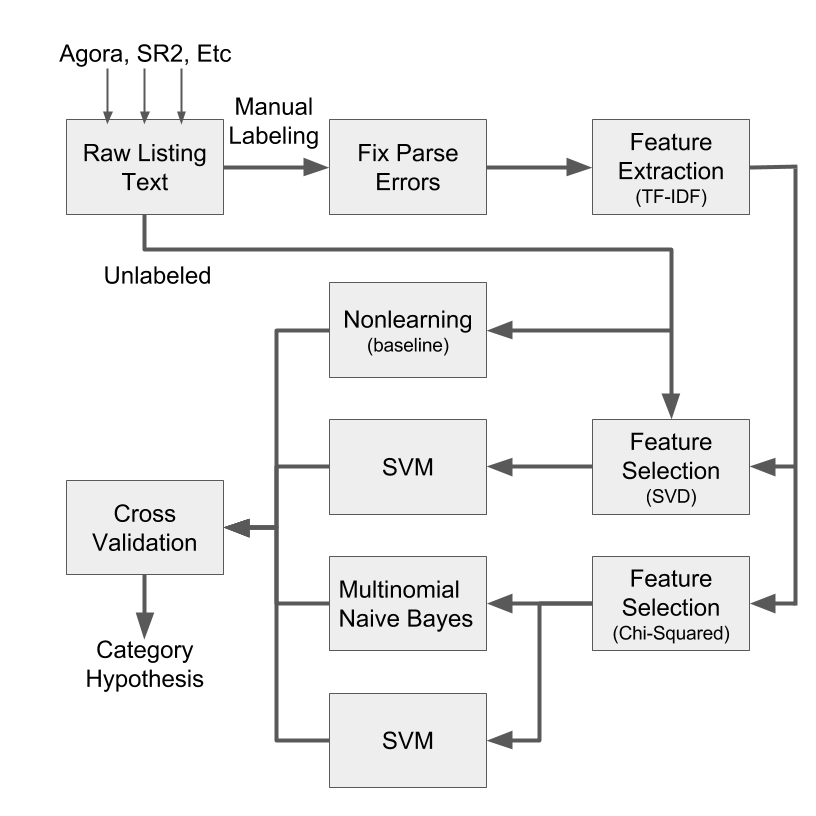
\includegraphics[width=0.85\linewidth]{pipeline}
        \caption{Data Pipeline}
    \end{center}
    \label{data_pipeline}
\end{figure}

We had $\frac{1}{3}$ of our data at the beginning of our algorithm design
process and had not used it for training or cross validation. We used our
processing pipeline to compute category predictions for each point the in test
set.

\subsection{Results}

The most important metric for our classification algorithm is categorization
accuracy. The accuracy for a test set is the proportion of labels that were
correctly assigned. For comparison, we compared the accuracy of our method with
three other algorithms.
\begin{itemize}
    \item A baseline model that used simple substring search, with substrings chosen by an online market expert.
					For example, if a product listing contained the text "xanax", then the listing was classified under "benzos".
    \item The $\chi^2$ test provides a simple way to remove features that are not correlated with any
					labeling, and is much faster than SVD.  However, it is also much less accurate and has a much higher output dimension than SVD.
    \item Multinomial Naive Bayes, using the same $\chi^2$ features.
\end{itemize}
The accuracy for each model is shown in Figure \ref{accuracy}. The figure shows
that our model outperformed several more simple models.

\begin{figure}[htbp]
    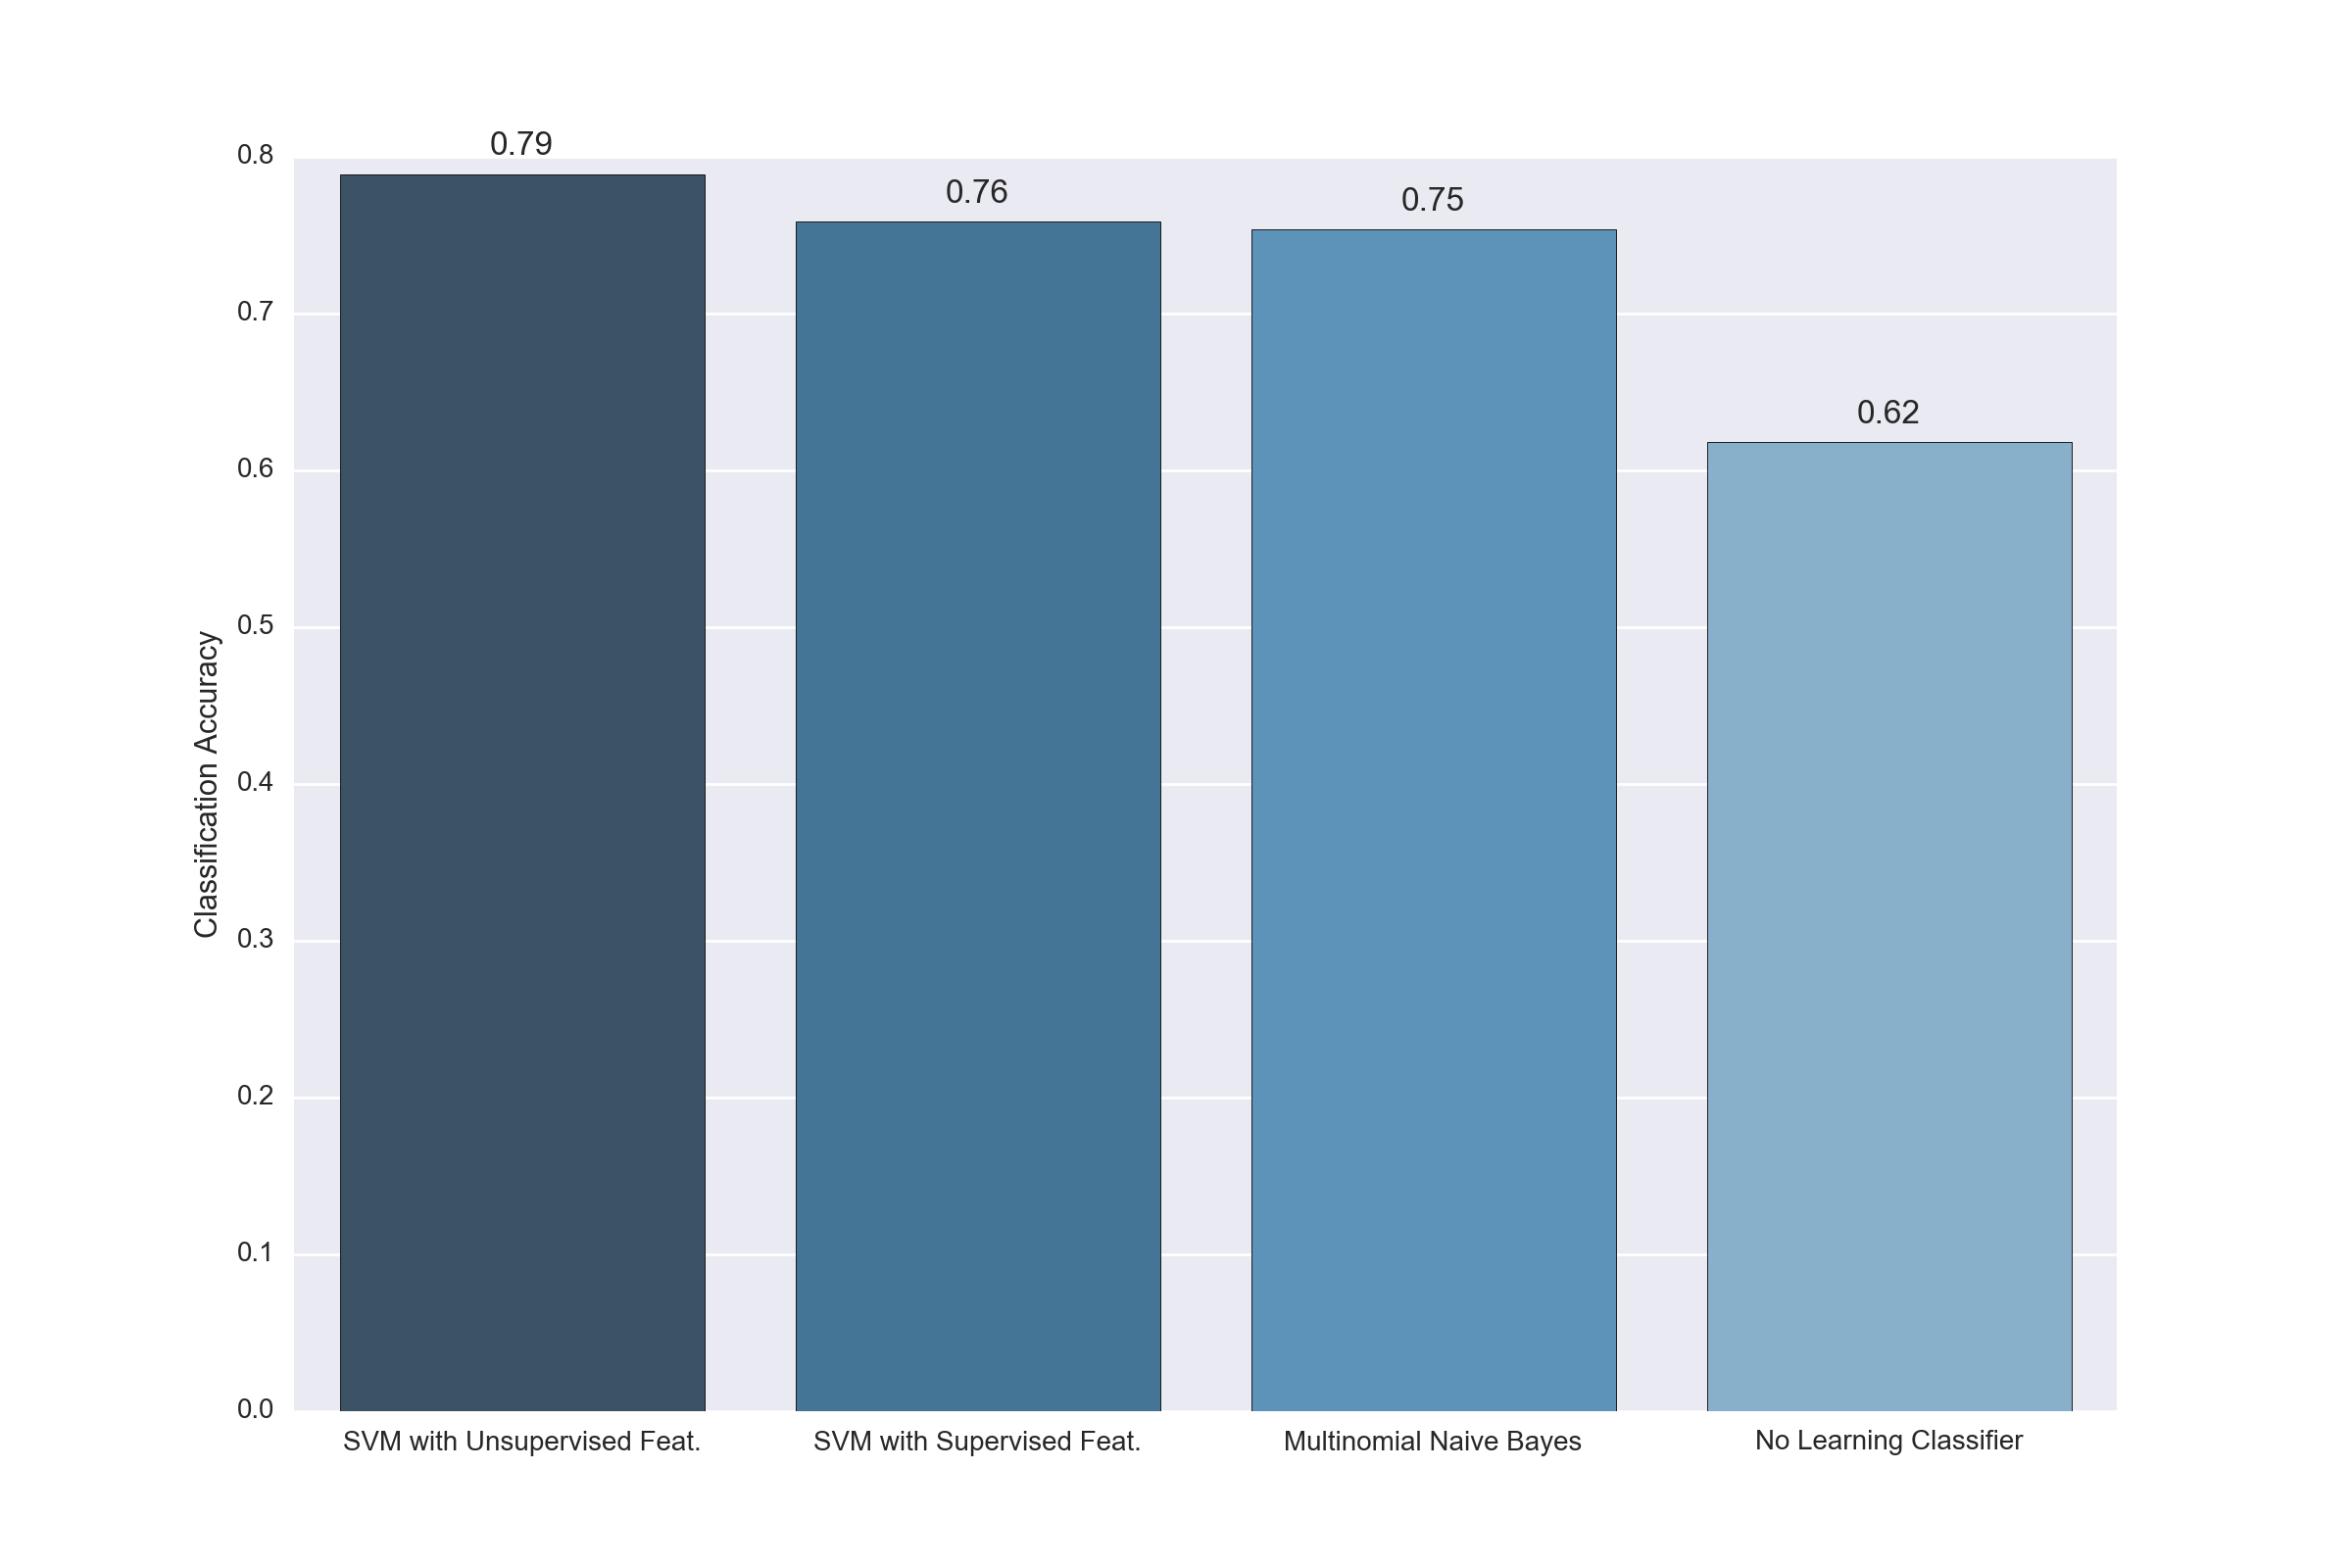
\includegraphics[width=\linewidth]{plots/models_accuracy}
    \caption{Comparison of Model Accuracies}
    \label{accuracy}
\end{figure}

\begin{table}[!ht]
    \begin{center}
        \begin{tabular}{| l | p{0.6\linewidth} |}
        \hline
        benzo & bensedin mot unmarked som bars 2mg diazepam xanax clonazepam zepose \\
        \hline
        dissociative &  purity reputation mxe 1000g methoxetamine chopping lab requested \\
        \hline
        ecstasy & 240 pressed pills mephedrone dutch red ecstasy express crystals 84 \\
        \hline
        misc & camel zolpidem lunesta eszopiclone caffeine phenargan zolab tranax  \\
        \hline
        opiate & 4mg 30mg heroine methadone opium codeine fentanyl naloxone tramadol \\
        \hline
        steroid & 10ml boldoject dianabol ml propionate sibutramine sibutramin test testosterone \\
        \hline
        psychedelic & buddha stand sheet babies mushrooms psilocybe hearts blotter nbome lsd \\
        \hline
        research chemical & fluoroamphetamine 36794 al 14g lad chiral dichloropane mdai fa apdb \\
        \hline
        prescription & mobic pseudoephedrine tadalafil generic dexamphetamine medications \\
        \hline
        stimulant & coke amphetamine check modafinil modalert adderall methamphetamine \\
        \hline
        marijuana & open grown dream crash kush weed hash wax taste sativa \\
        \hline
        other & size windows custom ways facebook account kinesiology book dpz guide \\
        \hline
        \end{tabular}
    \end{center}
    \caption{Top Tokens For Each Category}
    \label{category_tokens_table}
\end{table}



The precision recall curve compares shows the trade-off between precision (the
number of true positives over the total number of positives) vs recall (the
number of true positives over the number of true positives plus the false
negatives) as we vary our algorithm's parameters.
Figure \ref{prc_all} shows the precision-recall curve for our model.
\begin{figure}[htbp]
    \includegraphics[width=\linewidth]{plots/prc_all}
    \caption{Normalized Confusion Matrix}
    \label{prc_all}
\end{figure}

%%%%%%%%%%%%%%%%%%%%%%%%%%%%%%%%%%%%%%%%%%%%%%%%%%%%%%%%%%%%%%%%%%%%%%%%%%%%%%%%
% Confusion Matrix and discussion
\begin{figure}[htbp]
    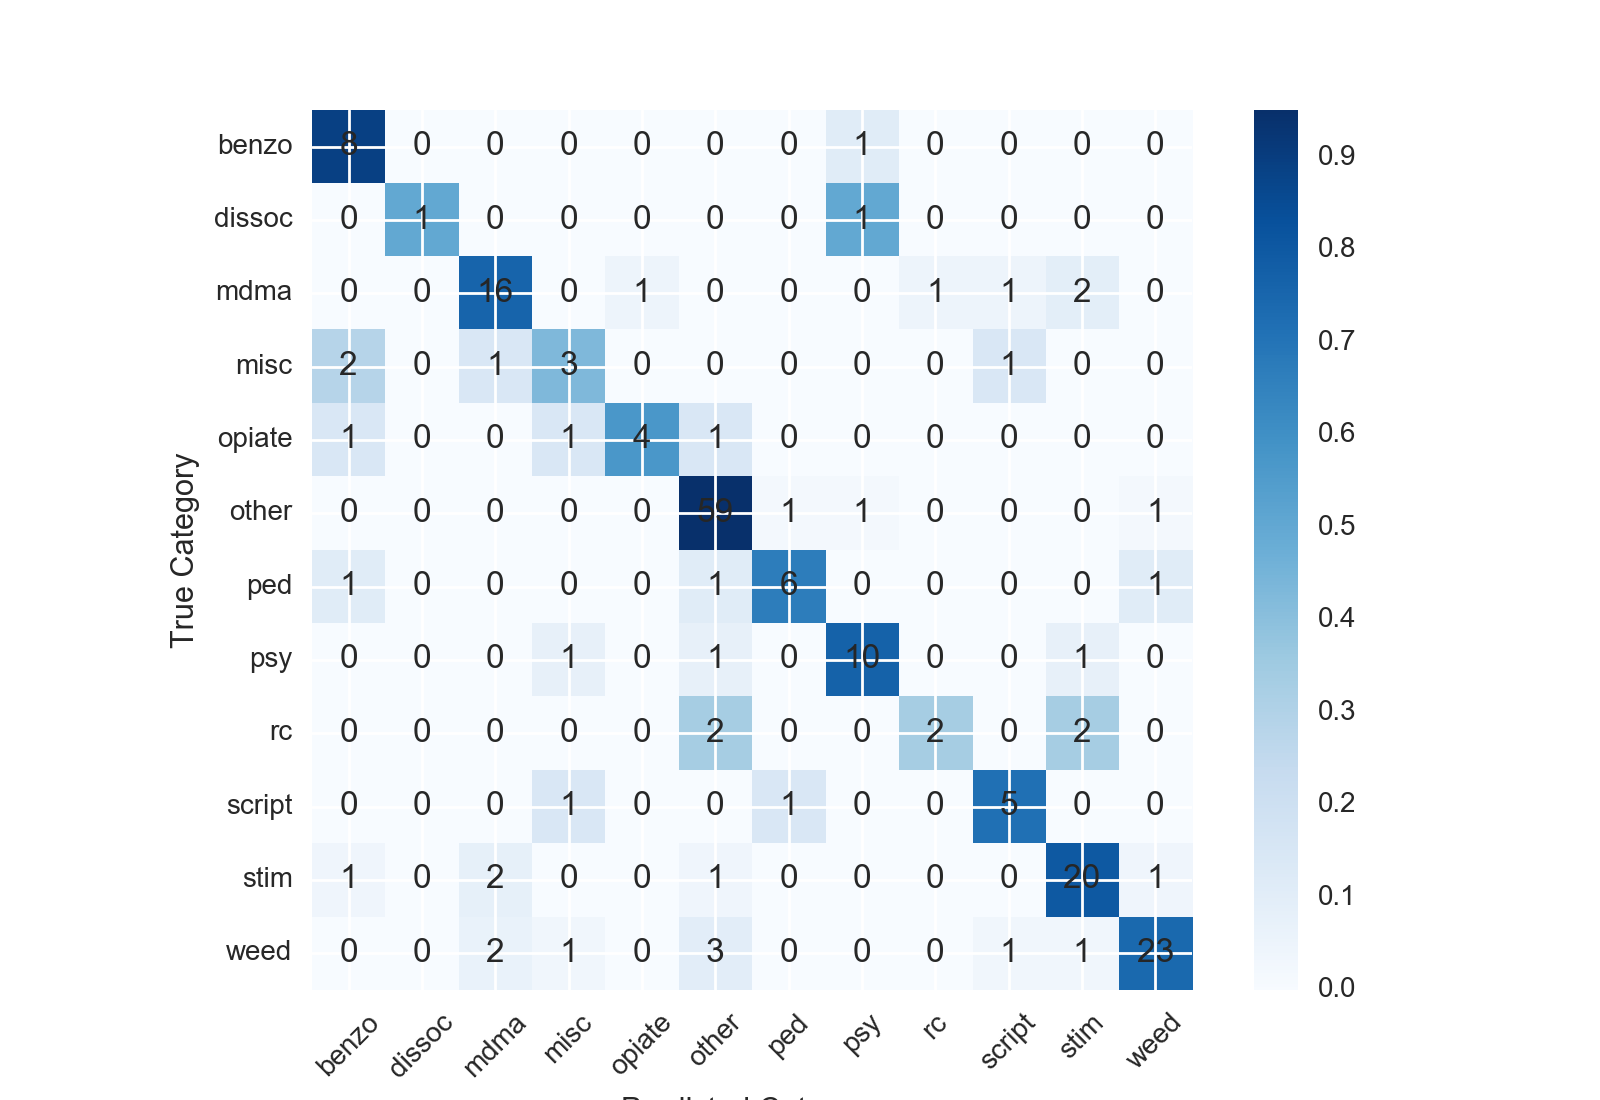
\includegraphics[width=\linewidth]{plots/confusion_matrix}
    \caption{Normalized Confusion Matrix}
    \label{confusion_matrix}
\end{figure}

Classification quality was not equal between each category. Figure \ref{confusion_matrix} shows the
confusion matrix of our algorithm on our test set. The grid position in row $i$ and column $j$ shows
the number of times a listing which is truly in category $i$ was classified by our algorithm as
category $j$. The values in the grid cells show the absolute number of test points, while the colors
show that number normalized by the true number of test points in each category.

The confusion matrix shows that our classifier was particularly bad at classifying the "other"
category.
We believe this is because of the large variety of "other" products available and the somewhat
arbitrary definition of the category. 
For example, we one category of goods we included in "other" was illegal digital goods, like movie downloads.
Because of this, drugs that had similar descriptions to unrelated products got misclassified as
"other".
To highlight this effect, our algorithm misclassified a strain of weed called "The Big Lebowski" as "other" because we had included a label for the movie download of "The Big Lebowski". See Table \ref{misclassified} for the complete example.

\begin{table}[!ht]
    \begin{center}
        \begin{tabular}{| l | p{0.6\linewidth} |}
        \hline
        True Category & Marijuana \\
        \hline
        Predicted Category & Other \\
        \hline
        Title & 1 4 Ounce The Big Lebowski \\
        \hline
        Description & The Big Lebowksi 2 3 week cure Indica sativa blend. Over the years pot has gotten a lot stronger especially with the advent of indoor hydroponic growing under metal halide and high pressure s...\\
        \hline
        \end{tabular}
    \end{center}
    \caption{Text of Typical Misprediction}
    \label{misclassified}
\end{table}


%%%%%%%%%%%%%%%%%%%%%%%%%%%%%%%%%%%%%%%%%%%%%%%%%%%%%%%%%%%%%%%%%%%%%%%%%%%%%%%%

% Did you do cross-validation, if so, how many folds? Before you list your results, make sure to
% list and explain what your primary metrics are: accuracy, precision, AUC, etc. Provide equations
% for the metrics if necessary. For results, you want to have a mixture of tables and plots. If you
% are solving a classification problem, you should include a confusion matrix or AUC/AUPRC curves.
% Include performance metrics such as precision, recall, and accuracy. You should have both
% quantitative and qualitative results. To reiterate, you must have both quantitative and
% qualitative results! This includes unsupervised learning (talk with your project TA on how to
% quantify unsupervised methods). Include visualizations of results, heatmaps, examples of where
% your algorithm failed and a discussion of why certain algorithms failed or succeeded. In addition,
% explain whether you think you have overfit to your training set and what, if anything, you did to
% mitigate that. Make sure to discuss the figures/tables in your main text throughout this section.
% Your plots should include legends, axis labels, and have font sizes that are readable when
% printed.
